\documentclass[conference]{IEEEtran}

\usepackage{pdfpages}

% correct bad hyphenation here
\hyphenation{op-tical net-works semi-conduc-tor}

\begin{document}
\title{Report for Wood's paper: 
The Feasibility of Magnetic Recording at 10 Terabits Per Square Inch on Conventional Media}

\author{\IEEEauthorblockN{Kamoliddin Mavlonov}
\IEEEauthorblockA{Graduate School of Science and Engineering\\
Ehime University\\
3 Bunkyou-cho Matsuyama Ehime 790-8577, Japan\\
kamol@koblab.cs.ehime-u.ac.jp}}

\maketitle

\begin{abstract}
This report is purely based on my own comprehension of this paper.
\end{abstract}

\IEEEpeerreviewmaketitle

\section{Introduction}
In 2000, Wood published a paper: The Feasibility of Magnetic Recording at 1 Terabits Per Square Inch~\cite{Wood}. It says, that conventional recording would reach a limit at around 1 Terabit/in^2.

However, current hard disk technology uses perpendicular recording, which already reaching this limit. TODO: find proof.
However, alternative technologies: heat-assisted magnetic recording (HAMR)~\cite{Rottmeyer} and bit patterned media (BPM)\cite{Terris}

\begin{figure}[!hbt]
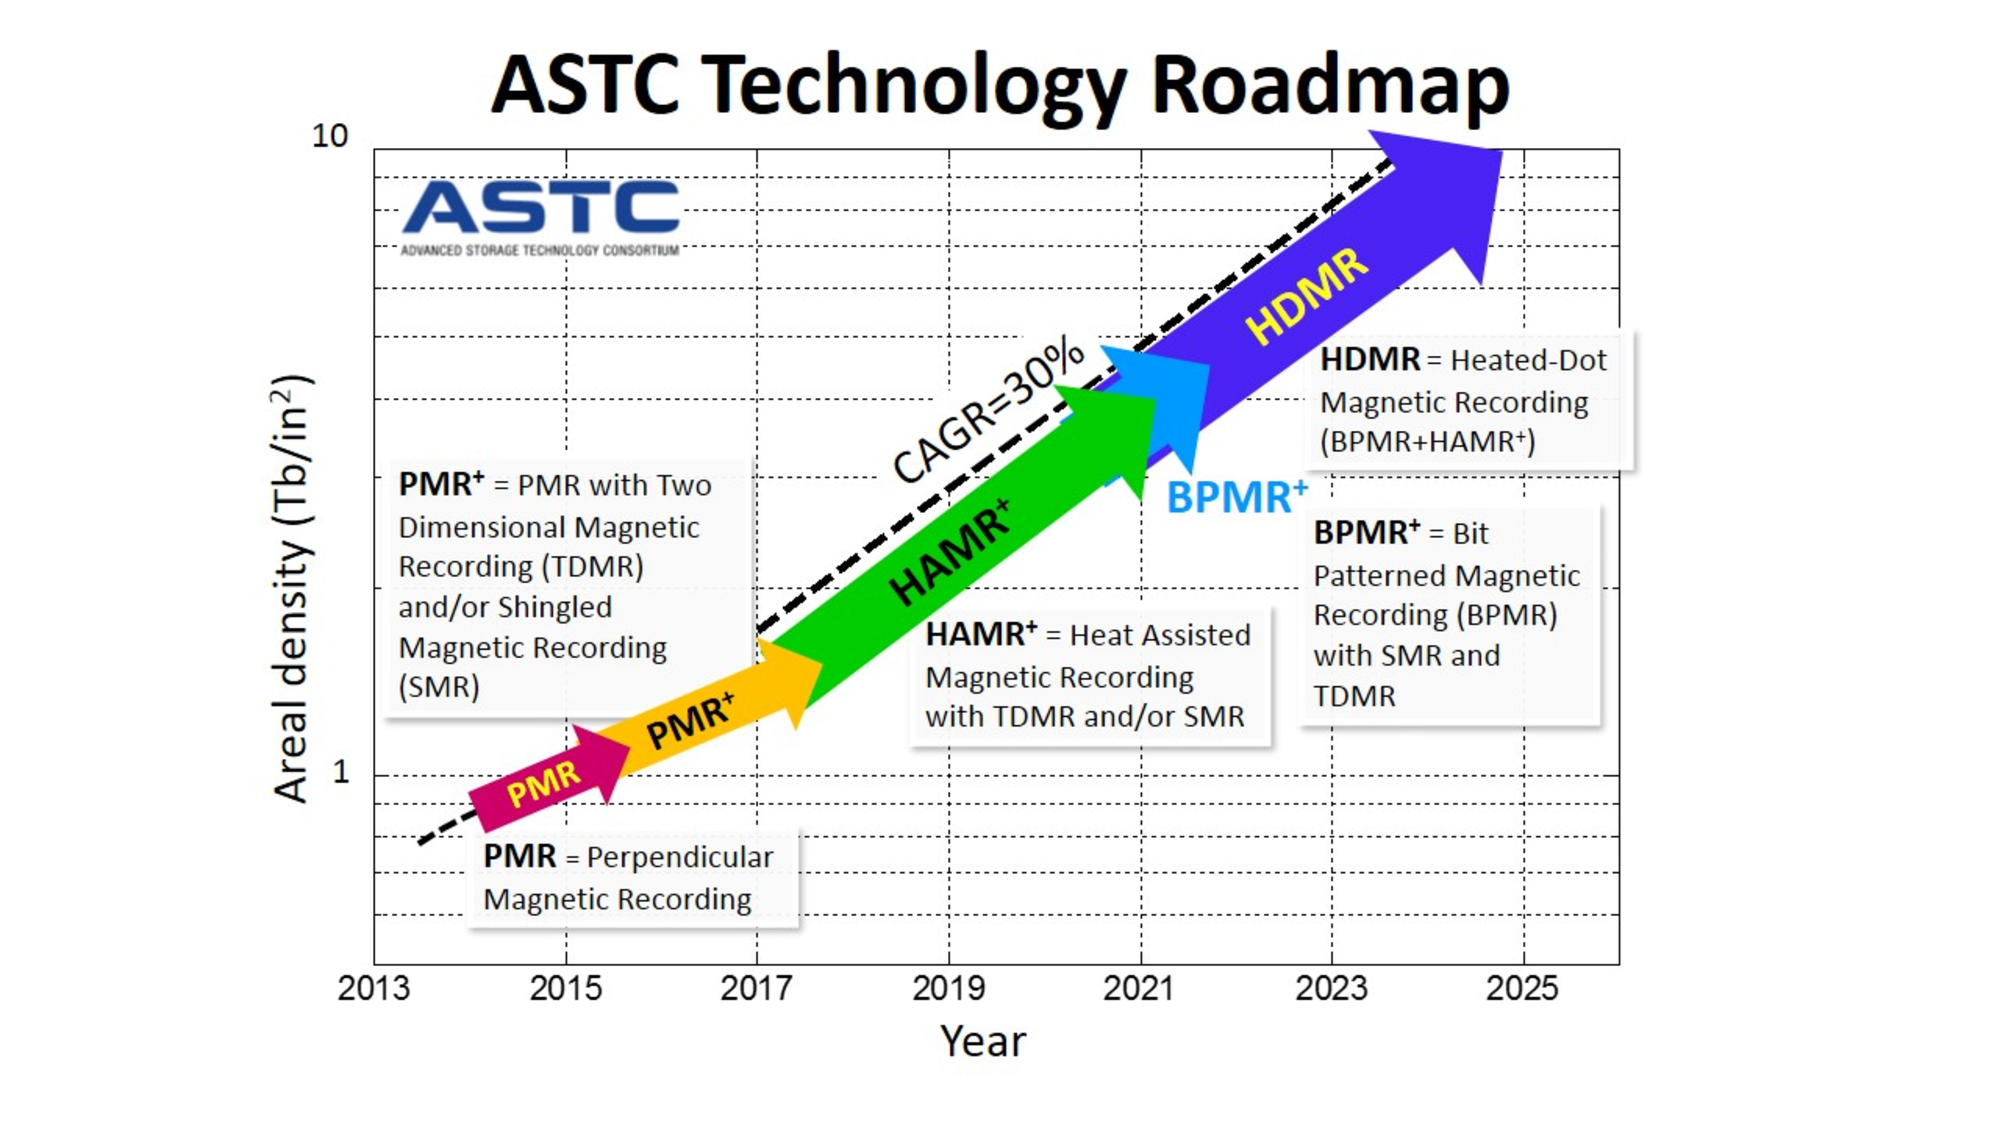
\includegraphics[height=0.25\textheight]{ASTC}
\caption{Data synchronization between two devices}
\label{fig_sync_no_conflict}
\end{figure}

\subsection{Subsection Heading Here}
Subsection text here.


\subsubsection{Subsubsection Heading Here}
Subsubsection text here.



\section{Conclusion}
The conclusion goes here.


% use section* for acknowledgment
\section*{Acknowledgment}


The authors would like to thank...

% set second argument of \begin to the number of references
% (used to reserve space for the reference number labels box)
\begin{thebibliography}{1}

\bibitem{Wood}
R.~Wood, \emph{The feasibility of magnetic recording at 1 terabit per square
inch}, IEEE Trans. Magn., vol. 36, pp. 36–42, Jan. 2000.

\bibitem{Rottmeyer}
R.~Rottmeyer et al., \emph{Heat-assisted magnetic recording}, IEEE Trans.
Magn., vol. 42, no. 10, pp. 2417–2421, Oct. 2006.

\bibitem{Terris}
B.~Terris, T. Thomson, and G. Hu, \emph{Patterned media for future magnetic
data storage}, Microsyst. Technol., vol. 13, no. 2, pp. 189–196, Nov.
2006.

\end{thebibliography}


% that's all folks
\end{document}